% Intended LaTeX compiler: pdflatex
\documentclass[final,anonym]{mcarticle}
% org-mc-latex.el ----------------------
\usepackage[utf8]{inputenc}
% extra (#+LaTeX_HEADER: lines) --------

% end of `org-latex-classes' -------------------------------------------------
\author{Fabrice NIESSEN}
\date{\today}
\title{Fichier de démo}
\hypersetup{
 pdfauthor={Fabrice Niessen},
 pdftitle={Fichier de démo},
 pdfkeywords={},
 pdfsubject={},
 pdfcreator={Emacs 26.1 (Org mode 9.0.9)}, 
 pdflang={Frenchb}}
\begin{document}

\maketitle

\chapter{Contexte}
\label{sec:org7b7d438}

\section{Nouveau}
\label{sec:nouveau}


\begin{enumerate}
\item préparer
\item chauffer
\item attendre
\end{enumerate}

Lorem \textsl{ipsum dolor sit} amet, consectetur adipisicing elit, sed do eiusmod
tempor incididunt \textsl{ut labore} et dolore magna aliqua. Ut enim ad minim veniam,

\begin{center}
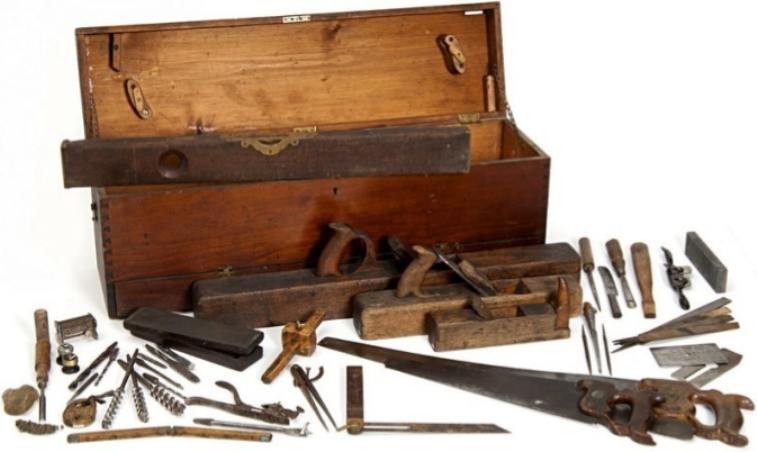
\includegraphics[width=.75\linewidth]{images/toolbox-messy.png}
\end{center}

\label{sec:org1e0b4ed}

quis nostrud exercitation ullamco laboris nisi ut aliquip ex ea commodo
consequat. Duis aute irure dolor in reprehenderit in voluptate velit esse

zearzaerzerzer
zaerzaerzaer
zaer
zaer
ze

\begin{table}[!htbp]
  \caption{\label{tab:org84e6251} Montants}
  \centering
  \begin{tabular}{lr}
      Montant & Mois      \\
      25      & resto     \\
      12      & cinema    \\
      21      & babysit   \\
  \end{tabular}
\end{table}

\begin{center}
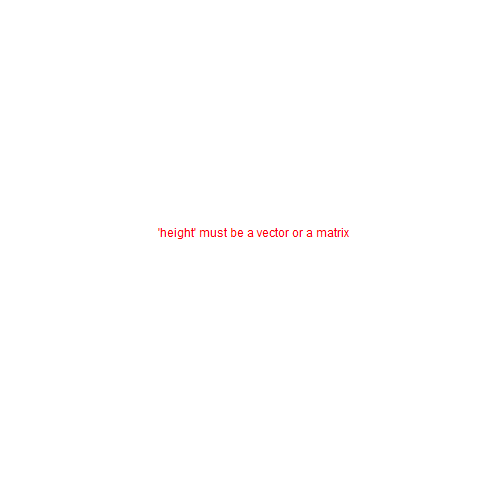
\includegraphics[width=.75\linewidth]{images/Rplots.png}
\end{center}

\section{Conclusions}
\label{sec:org2bf66a1}

cillum dolore eu fugiat nulla pariatur. Excepteur sint occaecat cupidatat non
proident, sunt in culpa qui officia deserunt mollit anim id est laborum.
\end{document}
